\section{Evaluating the Estimation Routine}
\label{sec:evaluation}

\subsection{\acs{1D} Datasets}
\label{subsec:onedim}

\subsubsection{``Twenty signals''}
\begin{sidewaysfigure}
    \centering
    \includegraphics{mpm_vs_nlp/mpm_vs_nlp.pdf}
    \caption[
        The result of estimating a series of 5 simulated signals comprising 20
        oscillators, using solely the \acs{MPM} and also with phase
        variance-regularised \acs{NLP} afterwards.
    ]{
        The result of estimating a series of 5 simulated signals comprising 20
        oscillators (see the main text for details on how the datasets were constructed).
        \textbf{a.} Spectra of the datasets generated.
        \textbf{b.} Spectral lines corresponding to the true set of oscillators
        used to generate each dataset.
        \textbf{c.} Plots of spectral lines for each oscillator generated using
        the \acs{MPM}.
        \textbf{d.} An equivalent plot for the result after applying \acs{NLP},
        with the \ac{MPM} result being the initial guess.
        Also included in \textbf{c.} and \textbf{d.} is the residual between the
        data and the sum of the oscillator peaks (grey line).
        The colouring of oscillator lines in \textbf{c.} and \textbf{d.} is
        described in the main text.
    }
    \label{fig:mpm_vs_nlp}
\end{sidewaysfigure}
In order to assess the estimation routine proposed in Chapter \ref{chap:theory}
-- specifically the effectiveness of applying \ac{NLP} using an initial guess
generated using the \ac{MPM} -- a series of synthetic \acp{FID} were constructed
using \eqref{eq:hypercomplex-fid} with $D=1$. For each \ac{FID}, a model order
of $M=20$ was used, the number of points sampled was $\None = 1024$, the sweep
width was $\fswone=\qty{125}{\hertz}$, and the transmitter offset was $\foffone
= \qty{0}{\hertz}$.  Each oscillator was assigned a phase of \ang{0}, while the
amplitudes, frequencies and damping factors were drawn at random from the
following distributions:
$\bdam \sim \mathcal{U}(1, 5)$, $\bdfonem \sim \mathcal{U}(\qty{-55}{\hertz},
\qty{55}{\hertz})$, $\bdetaonem \sim \mathcal{U}(\qty{2}{\per\second},
\qty{8}{\per\second})\ \forall m \in \lbrace 0, \cdots, 19\rbrace$. An extra
constraint was applied to the frequencies,
such that no two oscillators were permitted to have frequencies that differed
by less than $\nicefrac{4 \fswone}{\None} \approx \qty{0.49}{\hertz}$. Each
noiseless \ac{FID} was then corrupted with \ac{AWGN}, with a target \ac{SNR} of
\qty{25}{\deci\bel}\note{Reference that this is the lowest
SNR that the MPM considered to be effective}. The spectra of the simulated
\acp{FID} are presented in panel a of Figure \ref{fig:mpm_vs_nlp}, with the set
of true oscillator peaks in panel b.

For each \ac{FID}, the \ac{MPM} was performed, assuming that the model order is
30, constituting a considerable over-fit. The \ac{MDL} tended to produce
considerable under-estimates of $M$ are these \acp{FID}, so a hard-coded value
was used instead. Simulated signals featuring \ac{AWGN} typically show a
clean division between signal and noise components\note{better way of
describing this?}, with noise components
commonly being characterised by small amplitudes and/or very small damping
factors. For this reason, prior to subjecting the \ac{MPM} result to \ac{NLP},
oscillators which satisfied either $\bdam < 0.1$ or  $\bdetaonem <
\qty{0.7}{\per\second}$ were removed from the parameter set. The individual
oscillators which make up the \ac{MPM} result after purging noise components
are displayed in panel c of Figure \ref{fig:mpm_vs_nlp}, along with the
residual between the data and the summation of all the oscillator peaks (the
model).


The \ac{MPM} invariably generates a model with good agreement with the data, as
evidenced by the residual.
However, it can be seen that in several spectral regions across the datasets,
especially ones that are highly crowded, oscillators possess parameters which
deviate significantly from the true parameters, with the most notable feature
being individual oscillator phases -- these regularly stray far from \ang{0} --
and their associated amplitudes. The central motivation behind employing phase
variance-regularised \ac{NLP} is as a means of attempting to overcome this
detrimental feature of the \ac{MPM}.
In panel c of Figure \ref{fig:mpm_vs_nlp}, the blue oscillators are those which
agree very closely with a particular oscillator in the true set of parameters.
Oscillators with other colours are not clearly mapped to a true oscillator,
with the different colourings described shortly.
The intention is for the \ac{NLP} routine to adjust the parameters describing
the non-blue oscillators in panel c such that they agree with oscillators found
in the true set, while not affecting the blue oscillators.
The results of \ac{NLP} at convergence ($\epsilon = \num{1e-8}$) are provided
in panel d.

In discussing the outcome of the routine, it will be useful to introduce the
concept of a \emph{frequency neighbourhood}, a loose term which describes a
small, continuous range of frequencies within the spectral window. As the
\ac{NLP} routine involves taking small steps
through parameter space in an attempt to converge, it is unlikely that an
oscillator which starts off with a frequency far away from a particular
frequency neighbourhood will eventually enter it.  As such, in order for the
\ac{NLP} routine to successfully estimate the region, sufficient oscillators
need to present within the neighbourhood in the first place. Cases where the
\ac{MPM} generated enough oscillators for a given frequency neighbourhood,
albeit with parameters which are noticeably off the true parameters are in
either green or yellow. Green oscillators are those which the \ac{NLP} routine
was able to adjust in order to achieve agreement with the true result. As such,
they indicate improvements to the estimation result as opposed to the \ac{MPM}
being used by itself. Conversely, yellow oscillators denote cases where, though
sufficient oscillators exists in the frequency neighbourhood in the initial
guess, the \ac{NLP} routine evolves such that at least one of the oscillators
is driven by the phase variance constraint to acquire a negative amplitude,
such that it is purged from the parameter set. This typically occurs when an
oscillator has an initial phase which is considerably greater than \ang{90}.
Yellow oscillators therefore indicate cases where the final result has
under-fit the dataset. There are a few instances, denoted by red oscillators,
where the \ac{MPM} assigned too few oscillators to a particular frequency
region, and as such the \ac{NLP} would not have been able to yield any
improvement.
The final two oscillator groupings, denoted by purple and orange, denote cases
where the \ac{MPM} generated more oscillators than are present in a given
frequency neighbourhood (i.e. the data was over-fit in this region). Orange
oscillators we purged by the \ac{NLP} routine due to their acquiring negative
amplitudes. This enabled a parsimonious fit of th frequency neighbourhood by
the oscillators which remained. Finally, the purple oscillators denote the one
occasion where an over-fit occurred, and the model order was not successfully
reduced by the \ac{NLP} routine.

Overall, it can be seen that the inclusion of \ac{NLP} broadly improves the
output of the \ac{MPM}, where crowded regions often get assigned oscillators
with spurious complex amplitudes ($a$ and  $\phi$). \note{More discussion here...}

\subsubsection{Andrographolide}
Figure \ref{fig:andro-onedim} illustrates the outcome of applying the
estimation routine to selected regions of a \textsuperscript{1}H dataset of
andrographolide (Figure \ref{fig:structures}.e), in \acs{DMSOd6}. The \ac{NLP}
routine is effective at resolving the spurious phase-behaviour often generated
by the \ac{MPM}, while retaining reasonable fits to the data in most
circumstances. It's ability to estimate parameters from resonances with high
dynamic range is also evidenced by the fact that it was able to assign an
intense, broad singlet, corresponding to water, alongside a nearby quartet
corresponding the methylene in some residual ethanol in the sample.

Probably the most challenging aspect of estimating \ac{NMR} signals is
frequently being confronted with data that contains signals with incredibly
similar frequencies, with this dataset is a prime example. Andrographoilde has
a very dense coupling network, with some nuclei coupling to 4 or 5 other nuclei
with appreciable coupling constants. A prime example of this is spin (Q). This nucleus has separate 3-bond (vicinal) couplings to the diasteroetopic (M) and (N). Furthermore, it is likely to have small but appreciable four-bond couplings with the axial nuclei (P), (W) and (X), with the dihedral angle between (Q) and each of these being...

\begin{sidewaysfigure}
    \centering
    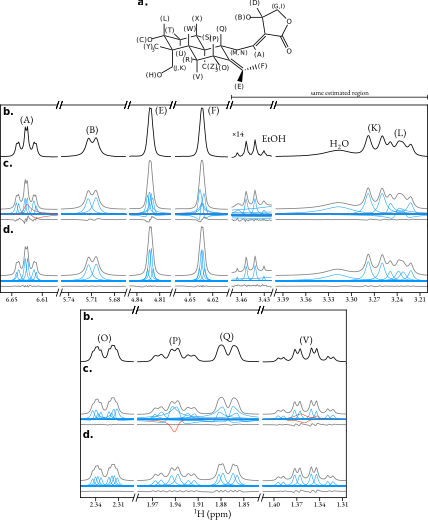
\includegraphics{andrographolide_onedim/andrographolide_onedim.pdf}
    \caption{
        Result of applying the estimation routine to a \ac{1D} dataset of andrographolide in \acs{DMSOd6}.
        \textbf{a.} Spectral data corresponding to the regions considered.
        \textbf{b.} The result of applying the \ac{MPM} to the regions, with
        the model order predicted with the \ac{MDL}. Blue/red lines: peaks of
        individual oscillators, grey line above: the model (sum of all
        oscillators), grep line below: the residual between the data and the model.
        \textbf{c.} The result after convergence of the \ac{NLP} routine, again
        with the model above and residual below.
        Red peaks in panel b correspond to oscillators which acquire negative
        amplitudes during the \ac{NLP} routine, and are subsequently purged.
        Note that one of the reasons estimated has been split in two in the
        figure to save space, with one half, featuring a signal from ethanol,
        being magnified.
    }
    \label{fig:andro-onedim}
\end{sidewaysfigure}
\note{TODO}
\begin{itemize}
    \item Figure \ref{fig:andro-onedim}.
    \item Able to resolve signals with considerable variation in damping
        (H\textsubscript{2}O vs (K), (L) signals, along with methylene quartet,
        which is immersed in the broad singlet).
    \item For particular multiplets, notably (P), (Q), residual provides
        evidence for under-fit: systematic ``wiggles'' in the residual imply
        single oscillator trying to fit frequency neighbourhood with more than
        one oscillator.
    \item Example illustrates considerable challenge in estimating datasets
        from molecules with very dense coupling networks (common with
        multi-cyclic molecules like andrographolide). (Q) provides extreme
        example of many small couplings leading to multiplet structures which
        are incredibly difficult to accurately resolve. Being an axial proton,
        4-bond couplings to other axial protons (P, W, X) are likely large
        enough to have an appreciable effect on lineshape (Karplus).
    \item Estimating (O) signal was more successful. Being equatorial, 4-bond
        couplings to other ring protons (\ang{60} dihedral angles) likely too
        small to be noticeable. Small residual implies parsimonius (i.e. no
        over-fit or under-fit) result: geminal coupling to (P), three-bond
        couplings to (R) and (V).
    \item (E/F): Small geminal alkene coupling.
\end{itemize}

